\chapter{Complexitat temporal}

\index{complexitat temporal}

L'eficiència dels algorismes és important en
la programació competitiva.
Normalment, és fàcil dissenyar un algorisme
que resol el problema lentament,
però el veritable repte és inventar un
algorisme que sigui ràpid.
Si l'algorisme és massa lent només obtindrem
punts parcials o cap punt.

La \key{complexitat temporal} d'un algorisme
és el temps, o nombre d'operacions, que l'algorisme necessita
per a resoldre entrades.
La idea és representar l'eficiència
com a una funció de la mida de l'entrada.
Quan calculem el cost d'un algorisme
podem esbrinar si serà prou ràpid
sense implementar-lo.

\section{Regles de càlcul}

La complexitat temporal d'un algorisme es denota per
$O(\cdots)$ on els punts suspensius representen alguna
funció.\footnote{Afegit: la complexitat temporal
d'un algorisme mesura com de ràpid creix el nombre
d'operacions que l'algorisme executa com més fem créixer
la mida de l'entrada. Formalment, la notació
$O(f(n))$ és el conjunt de funcions
que creixen com a molt tan ràpid com $f(n)$, llevat de
factors constants:
$O(f(n))=\{ g(n) | \exists n_0, c \forall n\ge n_0 \
g(n) \le c\cdot f(n) \}$.}
Normalment, la variable $n$ denota la mida de l'entrada.
Per exemple, si l'entrada és una matriu de
nombres, és usual prendre $n$ com la mida de la matriu,
i si l'entrada és una cadena de text, $n$ serà la mida
de la cadena.

\subsubsection*{Bucles}

Sovint els algorismes són lents
perquè contenen molts bucles que treballen amb l'entrada.
Com més bucles niats (bucles dintre d'altres bucles)
contingui l'algorisme, més lent és.
Si hi ha $k$ bucles niats, i cadascun d'ells fa $n$ iteracions,
la complexitat temporal és $O(n^k)$.

Per exemple, la complexitat temporal del codi següent és $O(n)$:
\begin{lstlisting}
for (int i = 1; i <= n; i++) {
    // codi O(1)
}
\end{lstlisting}

I la complexitat temporal del codi següent és $O(n^2)$:
\begin{lstlisting}
for (int i = 1; i <= n; i++) {
    for (int j = 1; j <= n; j++) {
        // codi O(1)
    }
}
\end{lstlisting}

\subsubsection*{Ordre de magnitud}

La complexitat temporal no ens diu el nombre exacte de vegades
que s'executa el codi dentre d'el bucle,
sinó l'ordre de magnitud.
En els exemples següents, el codi dins del bucle
s'executa $3n$, $n+5$ i $\lceil n/2 \rceil$ vegades,
però tots ells tenen complexitat de $O(n)$.

\begin{lstlisting}
for (int i = 1; i <= 3*n; i++) {
    // codi
}
\end{lstlisting}

\begin{lstlisting}
for (int i = 1; i <= n+5; i++) {
    // codi
}
\end{lstlisting}

\begin{lstlisting}
for (int i = 1; i <= n; i += 2) {
    // codi
}
\end{lstlisting}

En aquest altre example,
la complexitat temporal del codi següent és $O(n^2)$:

\begin{lstlisting}
for (int i = 1; i <= n; i++) {
    for (int j = i+1; j <= n; j++) {
        // codi
    }
}
\end{lstlisting}

\subsubsection*{Fases}

Si l'algorisme consta de fases consecutives,
la complexitat temporal és la complexitat temporal més
gran de les fases.
El motiu d'això és que la fase més lenta esdevé el
coll d'ampolla del codi.

Per exemple, el següent codi consta
de tres fases amb complexitats temporals
$O(n)$, $O(n^2)$ i $O(n)$.
Així, la complexitat total del temps és $O(n^2)$.

\begin{lstlisting}
for (int i = 1; i <= n; i++) {
    // codi
}
for (int i = 1; i <= n; i++) {
    for (int j = 1; j <= n; j++) {
        // codi
    }
}
for (int i = 1; i <= n; i++) {
    // codi
}
\end{lstlisting}

\subsubsection*{Diverses variables}

De vegades, la complexitat temporal depèn de
varis factors.
En aquest cas, podem expressar la complexitat temporal
com una fórmula de vàries variables.

Per exemple, la complexitat temporal del
el codi següent és $O(nm)$:

\begin{lstlisting}
for (int i = 1; i <= n; i++) {
    for (int j = 1; j <= m; j++) {
        // codi
    }
}
\end{lstlisting}

\subsubsection*{Recursió}

La complexitat temporal d'una funció recursiva depèn
del nombre de vegades que es crida la funció
multiplicat per la complexitat temporal d'una única crida.

Per exemple, considereu la funció següent:
\begin{lstlisting}
void f(int n) {
    if (n == 1) return;
    f(n-1);
}
\end{lstlisting}
La crida $\texttt{f}(n)$ provoca $n$ crides a funcions,
i la complexitat temporal de cadascuna d'aquestes crides
(sense comptar la crida recursiva) és $O(1)$.
Així, la complexitat total del temps és $O(n)$.

Com a altre exemple, considereu la funció següent:
\begin{lstlisting}
void g(int n) {
    if (n == 1) return;
    g(n-1);
    g(n-1);
}
\end{lstlisting}
En aquest cas, cada crida a la funció genera dues altres
crides, excepte quan $n=1$.
Vegem què passa quan es crida $g$
amb el paràmetre $n$.
La taula següent mostra el nombre de crides
produït per aquesta crida original:

\begin{center}
\begin{tabular}{rr}
crida de funció & nombre de crides \\
\hline
$g(n)$ & 1 \\
$g(n-1)$ & 2 \\
$g(n-2)$ & 4 \\
$\cdots$ & $\cdots$ \\
$g(1)$ & $2^{n-1}$ \\
\end{tabular}
\end{center}

En base a això, la complexitat temporal és
\[1+2+4+\cdots+2^{n-1} = 2^n-1 = O(2^n).\]

\section{Clases de complexitat}

\index{classes de complexitat}

El llistat següent conté les complexitats temporals
més comuns dels algorismes:

\begin{description}
\item[$O(1)$]
\index{algorisme de temps constant}
El temps d'execució d'un algorisme de \key{temps constant}
no depèn de la mida d'entrada.
Un algorisme típic de temps constant és una fórmula que
calcula la resposta directament.

\item[$O(\log n)$]
\index{algorisme logarítmic}
Un algorisme \key{logarítmic} sovint
divideix cada entrada per la meitat a cada pas.
El seu cost és logarítmic, perquè
$\log_2 n$ és igual al nombre de vegades que
és necessari dividir $n$ per 2 fins obtenir 1.

\item[$O(\sqrt n)$]
Un \key{algorisme d'arrel quadrada} és més lent que
$O(\log n)$ però més ràpid que $O(n)$.
Una propietat especial de les arrels quadrades és que
$\sqrt n = n/\sqrt n$, de manera que l'arrel quadrada
$\sqrt n$ està, en certa manera, a la meitat (geomètrica)
de l'entrada.

\item[$O(n)$]
\index{algorisme lineal}
Un algorisme \key{linial} és aquell que recorre l'entrada
un nombre constant de vegades.
Sovint aquesta és la millor complexitat temporal possible
en els concursos, perquè normalment cal accedir a cada
element de l'entrada com a mínim una vegada abans
de produir la resposta.

\item[$O(n \log n)$]
Aquest cost sovint indica que l'algorisme ordena l'entrada,
perquè aquest és el cost dels algorismes d'ordenació
eficients. Una altra possibilitat és que l'algorisme
utilitzi una estructura de dades on cada operació
triga $O(\log n)$ temps.

\item[$O(n^2)$]
\index{algorisme quadratic}
Un algorisme \key{quadratic} sovint conté
dos bucles niats un dintre de l'altre.
És possible passar per totes les parelles
d'elements de l'entrada en temps $O(n^2)$.

\item[$O(n^3)$]
\index{algorisme cúbic}
Un algorisme \key{cúbic} sovint conté
tres bucles niats.
És possible passar per totes les tripletes
d'elements de l'entrada en temps $O(n^3)$.

\item[$O(2^n)$]
Aquesta complexitat de temps sovint indica
que l'algorisme itera per tot
els subconjunts dels elements d'entrada.
Per exemple, els subconjunts de $\{1,2,3\}$ són
$\emptyset$, $\{1\}$, $\{2\}$, $\{3\}$, $\{1,2\}$,
$\{1,3\}$, $\{2,3\}$ i $\{1,2,3\}$.

\item[$O(n!)$]
Aquesta complexitat de temps sovint indica
l'algorisme itera per totes les
permutacions dels elements d'entrada.
Per exemple, les permutacions de $\{1,2,3\}$ són
$(1,2,3)$, $(1,3,2)$, $(2,1,3)$, $(2,3,1)$,
$(3,1,2)$ i $(3,2,1)$.

\end{description}

\index{algorisme polinomial}
Un algorisme és \key{polinòmic}
quan el seu cost és $O(n^k)$ per alguna constant $k$.
Tots els costos anteriors, exceptuant
$O(2^n)$ i $O(n!)$, són polinòmics.
A la pràctica, la constant $k$ sol ser petita,
i sovint s'associen costos polinòmics
amb que l'algorisme és \emph{eficient}.

\index{problema NP-difícil}

La majoria dels algorismes d'aquest llibre són polinòmics.
Tot i així, hi ha molts problemes importants per als quals
no es coneix cap algorisme polinòmic, és a dir,
ningú sap com resoldre'ls de manera eficient.
Els problemes \key{NP-hard} són un conjunt important
de problemes, per als quals no hi ha cap algorisme polinòmic
conegut\footnote{Un llibre clàssic sobre el tema és
de M. R. Garey i D. S. Johnson
\emph{Informàtica i intractabilitat: una guia per a la teoria
de NP-Completitud} \cite{gar79}.}.

\section{Estimació de l'eficiència}

Quan calculem la complexitat temporal
d'un algorisme podem comprovar,
abans d'implementar-lo, si és
prou eficient per al problema.
El punt de partida per les estimacions és el fet que
un ordinador modern pot realitzar alguns centenars de
milions d'operacions en un segon.

Per exemple, considerem un problema on el límit de temps
és d'un segon i la mida d'entrada és $n=10^5$.
Si la complexitat temporal és $O(n^2)$,
l'algorisme realitzarà unes $(10^5)^2=10^{10}$ operacions.
Això hauria de trigar almenys unes desenes de segons,
de manera que l'algorisme probablement sigui massa lent
per resoldre el problema.

D'altra banda, donada la mida de l'entrada,
podem intentar \emph{endevinar}
la complexitat de l'algorisme que hem de programar
per a resoldre el problema.
La taula següent conté algunes estimacions útils
suposant un límit de temps d'un segon. \footnote{No totes les operacions
costen el mateix: per exemple, les operacions d'entrada i sortida
són més costoses que les operacions aritmètiques.}

\begin{center}
\begin{tabular}{ll}
mida d'entrada & complexitat esperada \\
\hline
$n \le 10$ & $O(n!)$ \\
$n \le 20$ & $O(2^n)$ \\
$n \le 500$ & $O(n^3)$ \\
$n \le 5000$ & $O(n^2)$ \\
$n \le 10^6$ & $O(n \log n)$ o $O(n)$ \\
$n$ és gran & $O(1)$ o $O(\log n)$ \\
\end{tabular}
\end{center}

Per exemple, si la mida de l'entrada és $n=10^5$,
segurament la solució del problema sigui un
algorisme $O(n)$ o $O(n \log n)$.
Aquesta informació facilita el disseny de l'algorisme,
perquè descarta enfocaments que donarien
un algorisme amb un cost massa gran.

\index{factor constant}

Tot i així, és important recordar que
la complexitat temporal és només una estimació de l'eficiència,
perquè amaga els \emph{factors constants}.
Per exemple, un algorisme que s'executa en $O(n)$ temps
potser fa $n/2$ o $5n$ operacions.
Això és un factor important de cara al temps
real que farà servir l'algorisme.

\section{Suma màxima d'un subvector}

\index{suma màxima d'un subvector}

Sovint hi ha diversos algorismes
que poden resoldre un problema i que tenen distintes
complexitats temporals.
Aquesta secció tracta d'un problema clàssic que
té una solució $O(n^3)$ senzilla.
Tanmateix, dissenyant un algorisme millor, 
és possible resoldre el problema en temps $O(n^2)$
temps o fins i tot en temps $O(n)$.

Donat un vector de $n$ nombres,
la nostra tasca és calcular el
\key{suma màxima d'un subvector}, és a dir,
la suma més gran possible d'una
seqüència de valors consecutius
del vector\footnote{El llibre \emph{Programming Pearls} \cite{ben86} de J. Bentley va popularitzar aquest problema.}.
El problema és interessant quan hi ha valors
negatius en el vector.
Per exemple, en el vector
\begin{center}
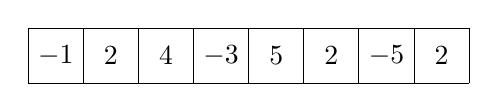
\begin{tikzpicture}[scale=0.7]
\draw (0,0) grid (8,1);

\node at (0.5,0.5) {$-1$};
\node at (1.5,0.5) {$2$};
\node at (2.5,0.5) {$4$};
\node at (3.5,0.5) {$-3$};
\node at (4.5,0.5) {$5$};
\node at (5.5,0.5) {$2$};
\node at (6.5,0.5) {$-5$};
\node at (7.5,0.5) {$2$};
\end{tikzpicture}
\end{center}
\begin{samepage}
el subvector següent té suma màxima $10$:
\begin{center}
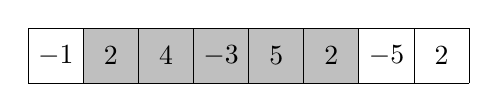
\begin{tikzpicture}[scale=0.7]
\fill[color=lightgray] (1,0) rectangle (6,1);
\draw (0,0) grid (8,1);

\node at (0.5,0.5) {$-1$};
\node at (1.5,0.5) {$2$};
\node at (2.5,0.5) {$4$};
\node at (3.5,0.5) {$-3$};
\node at (4.5,0.5) {$5$};
\node at (5.5,0.5) {$2$};
\node at (6.5,0.5) {$-5$};
\node at (7.5,0.5) {$2$};
\end{tikzpicture}
\end{center}
\end{samepage}

Suposem que es permet triar un subvector buit,
de manera que la suma màxima és sempre com a mínim $0$.

\subsubsection{Algorisme 1}

Una manera senzilla de resoldre el problema
és passar per tots els subvectors possibles,
calcular la suma de valors de cada subvector i mantenir
la suma màxima.
El codi següent implementa aquest algorisme:

\begin{lstlisting}
int millor = 0;
for (int a = 0; a < n; a++) {
    for (int b = a; b < n; b++) {
        int suma = 0;
        for (int k = a; k <= b; k++) {
            suma += v[k];
        }
        millor = max(millor,suma);
    }
}
cout << millor << "\n";
\end{lstlisting}

Les variables \texttt{a} i \texttt{b} contenen el primer i
el darrer índex del subvector,
i la suma de valors es calcula a la variable \texttt{suma}.
La variable \texttt{millor} conté la suma màxima trobada
durant la cerca.

La complexitat temporal de l'algorisme és $O(n^3)$,
perquè consta de tres bucles niats
que recorren l'entrada.

\subsubsection{Algorisme 2}

És fàcil fer que l'algorisme 1 sigui més eficient
eliminant-ne un bucle.
Això és possible si calculem la suma a la vegada que moguem
el darrer índex del subvector.
El resultat és el codi següent:

\begin{lstlisting}
int millor = 0;
for (int a = 0; a < n; a++) {
    int suma = 0;
    for (int b = a; b < n; b++) {
        suma += v[b];
        millor = max(millor, suma);
    }
}
cout << millor << "\n";
\end{lstlisting}
Després d'aquest canvi, la complexitat temporal és $O(n^2)$.

\subsubsection{Algorisme 3}

Sorprenentment, és possible\footnote{En \cite{ben86}, aquest algorisme de
temps lineal s'atribueix a J. B. Kadane, i l'algorisme de
vegades s'anomena \index{algorisme de Kadane}
\key{algorisme de Kadane}.} resoldre el problema
en temps $O(n)$, que significa que n'hi ha prou amb un sol bucle.
La idea és calcular, per a cada posició del vector,
la suma màxima d'un subvector que acaba en aquesta posició.
Després d'això, la resposta al problema és el
màxim d'aquestes sumes.

Considereu el subproblema de trobar la suma màxima del
subvector que acaba a la posició $k$.
Hi ha dues possibilitats:
\begin{enumerate}
\item El subvector només conté l'element a la posició $k$.
\item El subvector consisteix en un subvector que acaba
a la posició $k-1$, seguit de l'element a la posició $k$.
\end{enumerate}

En aquest darrer cas, ja que volem
trobar un subvector amb suma màxima,
el subvector que acaba a la posició $k-1$
també ha de tenir suma màxima.
Així, podem resoldre el problema de manera eficient
calculant la suma màxima del subvector
per a cada posició final d'esquerra a dreta.

El codi següent implementa l'algorisme:
\begin{lstlisting}
int millor = 0, suma = 0;
for (int k = 0; k < n; k++) {
    suma = max(v[k],sum+v[k]);
    millor = max(millor, suma);
}
cout << millor << "\n";
\end{lstlisting}

L'algorisme només conté un bucle
que passa per l'entrada,
per tant, la complexitat temporal és $O(n)$.
Aquesta és també la millor complexitat temporal possible,
perquè qualsevol algorisme per aquest problema
ha d'examinar tots els elements del vector almenys una vegada.

\subsubsection{Comparació d'eficiència}

És interessant estudiar com d'eficients són
els algorismes a la pràctica.
La taula següent mostra els temps de funcionament
dels algorismes anteriors per a diferents
valors de $n$ en un ordinador modern.

En cada prova, vam generar l'entrada aleatòriament, i
no vam mesurar el temps necessari per llegir l'entrada.

\begin{center}
\begin{tabular}{rrrr}
mida del vector $n$ & algorisme 1 & algorisme 2 & algorisme 3 \\
\hline
$10^2$ & $0.0$ s & $0.0$ s & $0.0$ s \\
$10^3$ & $0.1$ s & $0.0$ s & $0.0$ s \\
$10^4$ & > $10.0$ s & $0.1$ s & $0.0$ s \\
$10^5$ & > $10.0$ s & $5.3$ s & $0.0$ s \\
$10^6$ & > $10.0$ s & > $10.0$ s & $0.0$ s \\
$10^7$ & > $10.0$ s & > $10.0$ s & $0.0$ s \\
\end{tabular}
\end{center}

La comparació mostra que tots els algorismes
són eficients quan la mida de l'entrada és petita,
però les entrades més grans mostren diferències
notables entre els temps d'execució dels algorismes.
L'algorisme 1 es torna lent
quan $n=10^4$, i l'algorisme 2
es torna lent quan $n=10^5$.
Només l'algorisme 3 pot processar
fins i tot les entrades més grans instantàniament.
